\chapter{Análise Bibliográfica sobre Cálculo Lambda, por Leonardo Alves Riether\label{chap:bibliometria:LeoRiether}}

\section{Planejamento do estudo}
O lambda cálculo, ou cálculo-$\lambda$, é um modelo computacional tão poderoso quanto a Máquina de Turing, mas com certas propriedades que o deixam mais elegante e fácil de analisar. Algumas dessas propriedades, como descrito por \citet{lynn_lambda_nodate}, são a simplicidade, praticidade e correção. Por conta disso, várias linguagens funcionais, como Haskell e Kind\citep{kindelia_kind_nodate}, são baseadas nesse modelo de computação.

Com a atual tendência de linguagens de programação implementarem cada vez mais recursos funcionais, é possível que avanços na teoria do cálculo-$\lambda$ tragam benefícios práticos para essas linguagens, o que pode incentivar o estudo dessa área do conhecimento pelos pesquisadores.

É interessante, portanto, analisar o que já foi publicado sobre esse cálculo, de forma a extrair métricas sobre a história e evolução da área ao longo do tempo.

Com base nisso, este trabalho objetivou responder as seguintes perguntas:
\begin{itemize}
    \item Como é o histórico do nível de intensidade de publicações sobre cálculo-$\lambda$ da comunidade científica? Os pesquisadores estão mais interessados nele agora que no passado, ou menos? 
    \item Quais são os países e instituições que mais produzem conteúdo científico sobre o cálculo lambda? 
    \item Quais são os termos mais importantes relacionados a esse sistema computacional?
\end{itemize}

\subsection{O que já existe de pesquisa bibliométrica sobre esse tema?}
Pesquisas na Web of Science, SCOPUS e Google Scholar não encontraram resultados relevantes, portanto não foi possível encontrar nenhuma pesquisa bibliométrica sobre o cálculo-$\lambda$ feita anteriormente.

\subsection{Uso do Bibliometrix e Biblioshiny}
O estudo será feito com auxílio das ferramentas Bibliometrix e Biblioshiny, executados por meio do RStudio, conforme o \textit{worflow} recomendado pelos autores do pacote, indicado na figura ~\ref{fig:bibliometrix:workflow}.

\subsection{Limitações}
A pesquisa foi realizada no período de uma semana, e portanto não foi possível analisar muito a fundo. Além disso, a única base de dados utilizada foi a Web of Science, mantida pela Clarivate. Em um estudo posterior, seria interessante ter mais tempo para fazer a pesquisa e utilizar mais de uma base de dados bibliográficos.


\section{Coleta de dados\label{leoriether:lammetrics:coleta}}
Os dados obtidos foram coletados utilizando a ferramenta Web of Science, da Clarivate, no dia 08 de fevereiro de 2022, acessada por meio do Portal de Periódicos da CAPES. A coleção utilizada foi a Science Core Collection, edição Science Citation Index Expanded (SCI-EXPANDED), que possui artigos indexados desde 1945 sobre as áreas de ciências exatas e naturais.

\lstinputlisting[numbers=left,basicstyle=\normalsize\ttfamily,caption={\query\  de busca no WoS sobre lambda cálculo},label=leoriether-lammetrics-query]{experiments/LeoRiether/AnaliseBibliometrica/LambdaCalculus/WoS-20220208/query.txt}

Com isso, foram obtidos 2612 registros bibliográficos sobre o cálculo-$\lambda$, incluindo algumas de suas variantes, como o cálculo mu-lambda, o cálculo-$\lambda$ não tipado e o com tipagem simples. Após exportação dos registros em blocos de até mil itens, com a opção \textit{Exportar registros para arquivo de texto sem formatação}, os arquivos foram concatenados, formando um arquivo de 7.99MB com todos os dados, que pode ser encontrado no GitHub da disciplina, em \url{https://github.com/jhcf/Comput-Experim-20212/blob/main/experiments/LeoRiether/AnaliseBibliometrica/LambdaCalculus/WoS-20220208/recs.txt}.

\subsection{Explicação da \query de Busca}
Como o objetivo era analisar todas as publicações relacionadas ao estudo do lambda cálculo, a query utilizada na Web of Science utiliza as palavras chave "lambda" e "calculus", ou "calculi". A pesquisa, porém, foi limitada a categorias de Matemática, Lógica e Computação, a fim de omitir resultados relacionados à Física. A query produzida é mostrada na listagem \ref{leoriether-lammetrics-query}.

\section{Análise dos dados}

\subsection{Filtragem de registros}
Foi aplicado um filtro ao \dataset\  inicial, que possuia 2612 registros, para que a análise fosse feita apenas em registros de artigos publicados em revistar científicas, assumindo que o conhecimento científico publicado nessas revistas é mais rigoroso. Após a filtragem, obtivemos 1787 registros de artigos sobre o Lambda Cálculo, que serão chamados de LC@LeoRiether.

\subsection{Análise descritiva do \dataset\   LC@LeoRiether}

A primeira análise a ser feita é a análise descritiva do \dataset\  LC@LeoRiether. Para isso, abrimos no Biblioshiny a seção \textit{Dataset > Main Information}, que calcula as informações necessárias. A partir diss, conseguimos as seguintes informações gerais sobre o dataset:

\begin{description}
    \item [\textit{Timespan}] Os artigos encontrados pela query no Web of Science datam desde 1970 até 2022.
    \item [\textit{Sources (Journals, Books, etc)}] Foram encontradas 311 fontes de informação que publicaram artigos presentes no \dataset\ LC@LeoRiether. Assim, cada fonte publicou em média $\frac{1787}{311} =5.75$ artigos.
    \item [\textit{Average years from publication}] A média do tempo de publicação dos artigos no dataset foi de 14.5 anos.
    \item [\textit{Average citations per documents}] Cada documento foi citado, em média, 12.33 vezes.
    \item [\textit{Average citations per year per doc}] Cada documento foi citado, em média, 0.9031 vezes por ano.
    \item [\textit{References}] O \dataset\  LC@LeoRiether possui 33701 referências citadas (tags CR)
    \item [\textit{Keywords Plus (ID)}] Foram encontradas 1538 palavras-chave distintas do tipo Keywords Plus (ID).
    \item [\textit{Author's Keywords (DE)}] Foram encontradas 3341 palavras-chave distintas indicadas pelas autores.
    \item [\textit{Authors}] 2259 nomes de autores distintos estão presentes no \dataset\  LC@LeoRiether.
    \item [\textit{Author Appearances}] Os 2259 distintos (nomes de) autores foram encontrados 3560 vezes, como autores de artigos.
        
    \item [\textit{Authors of single-authored documents}] Há 513 autores, dentre os 2259 autores do \dataset\  , que editaram publicações individualmente
    \item [\textit{Authors of multi-authored documents}] Há 1746 autores, dentre os 2259 autores do \dataset\  , que editaram publicações com um ou mais co-autores
    \item [\textit{Single-authored documents}] Dentre os 1787 documentos do \dataset\  LC@LeoRiether, 672 deles foram escritos por um autor individualmente, enquanto os outros 1115 foram escritos colaborativamente.
    \item [\textit{Documents per Author}] Em média, cada autor publicou 0.791 documentos.
    \item [\textit{Authors per Document}] Em média, cada documento foi produzido por 1.26 autores.
    \item [\textit{Co-Authors per Documents}] No \dataset\ LC@LeoRiether, há uma média de 1.99 co-autores por artigo publicado.
    \item [\textit{Collaboration Index}] O índice de colaboração encontrado no \dataset\  LC@LeoRiether é de 1.57.
\end{description}

\subsection{Evolução da Produção Científica}
Com o Bibliometrix, podemos analisar como a produção científica de artigos sobre o cálculo-$\lambda$ evoluiu ao longo dos anos, segundo o \dataset\  LC@LeoRiether. Ao realizar essa análise, encontramos a imagem \ref{fig:evol:anual:LC@LeoRiether}. 

\begin{figure}
    \centering
    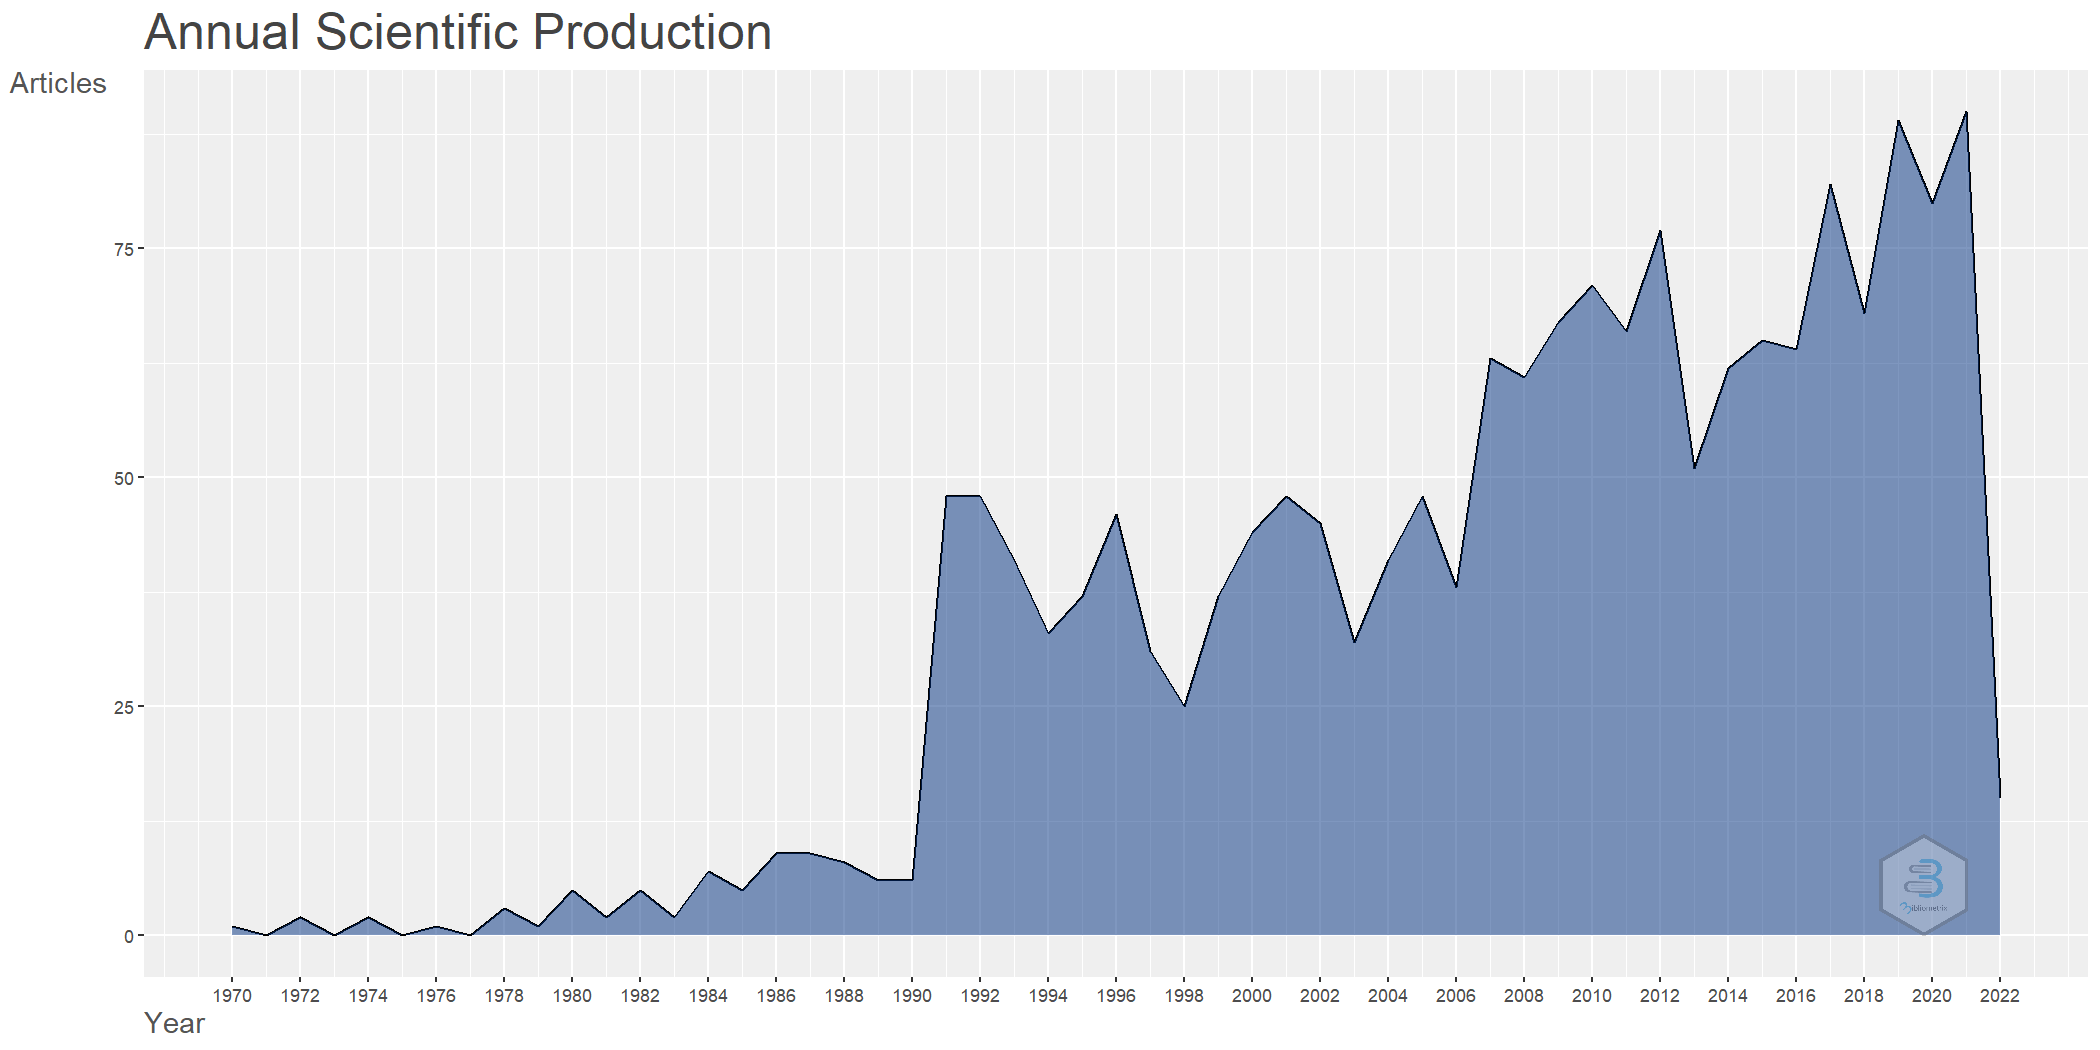
\includegraphics[width=1\textwidth]{experiments/LeoRiether/AnaliseBibliometrica/LambdaCalculus/WoS-20220208/Images/AnnualScientificProduction.png}
    \caption{Evolução da produção científica no \dataset\   LC@LeoRiether.}
    \label{fig:evol:anual:LC@LeoRiether}
\end{figure}

O \textit{Annual Growth Rate} encontrado no \dataset\  LC@LeoRiether é de 5.8\%, levemente maior que a taxa de crescimento anual da publicação científica mundial, de cerca de 3.3\%.

\subsection{Interpretação do Crescimento}
Há dois pontos interessantes que podemos observar no gráfico \ref{fig:evol:anual:LC@LeoRiether}. O primeiro deles é como a produção científica nessa área de estudo subiu abruptamente a partir de 1991, possivelmente indicando uma descoberta importante que levou a um grande aumento de interesse da comunidade. O segundo ponto é que, diferentemente de gráficos de evolução de produção científica de algumas outras áreas, não há um aumento exponencial no número de publicações por ano -- esse aumento é mais lento e contínuo.

\subsection{Evolução das Citações}
Outra análise que pode ser feita sobre o \dataset\  LC@LeoRiether é a de evolução de citações. A figura \ref{fig:evol:anual:citacoes:LC@LeoRiether} mostra os resultados obtidos a partir dessa análise.

\begin{figure}
    \centering
    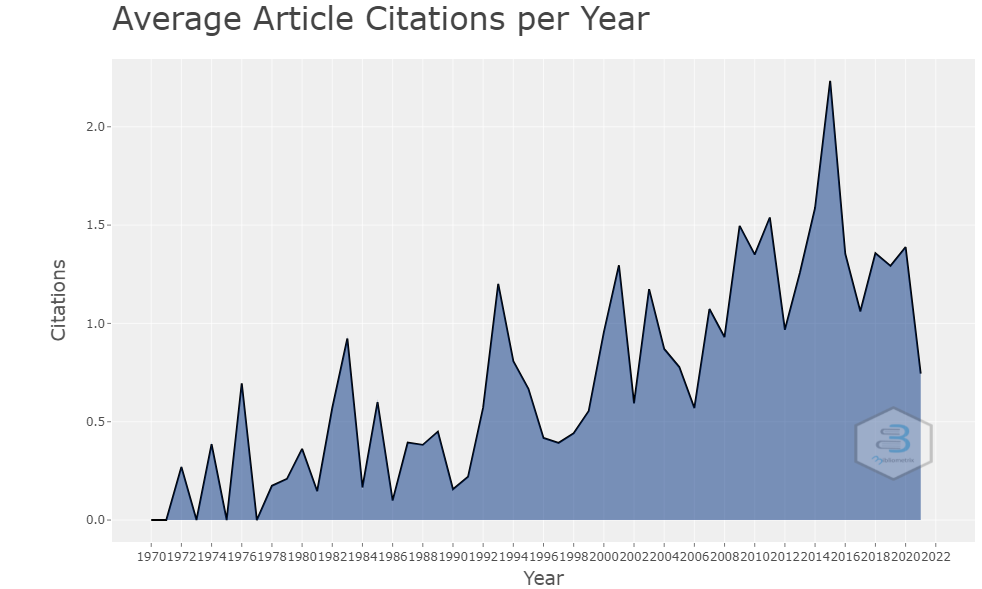
\includegraphics[width=1\textwidth]{experiments/LeoRiether/AnaliseBibliometrica/LambdaCalculus/WoS-20220208/Images/AverageCitationsPerYear.png}
    \caption{Evolução das citações ao \dataset\   LC@LeoRiether.}
    \label{fig:evol:anual:citacoes:LC@LeoRiether}
\end{figure}

Com base na figura, observamos que há um crescimento aproximadamente constante, porém pequeno, de citações por ano. Note que o eixo de média de citações por ano não tem uma grande extensão, indo de 0 citações até um máximo de somente 2.2, em 2015. Além disso, vemos, como no gráfico de produção científica anual da figura \ref{fig:evol:anual:LC@LeoRiether} da seção anterior, um pico de média de citações entre 1991 e 1993. Dessa vez, no entanto, esse pico é seguido de uma queda no número de citações até 1997.

\subsection{\textit{Three-Field Plots (Sankey diagram)}}

\begin{figure}
    \centering
    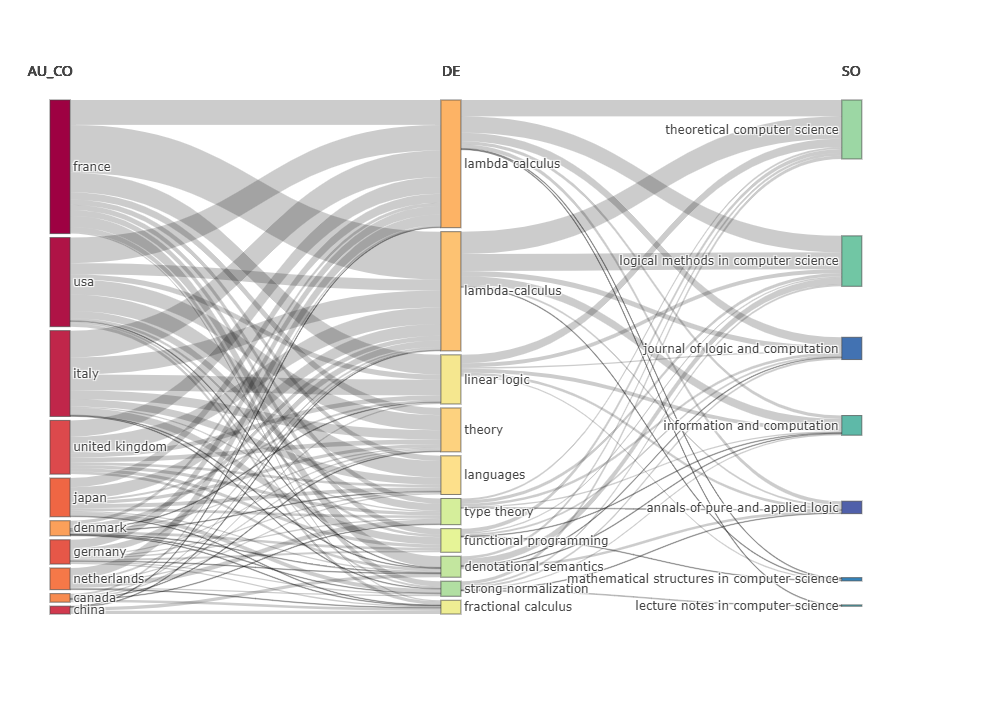
\includegraphics[angle=0,width=1\textwidth]{experiments/LeoRiether/AnaliseBibliometrica/LambdaCalculus/WoS-20220208/Images/ThreeFieldsPlot.png}
    \caption{Plotagem ``Três Campos'' (Sankey plot) do \dataset\   LC@LeoRiether: 10 Países, Palavras-Chave e Revistas.}
    \label{fig:LC@LeoRiether:ThreeFieldPlot}
\end{figure}

Outra visualização que podemos fazer sobre o \dataset\  LC@LeoRiether é uma Plotagem de Três Campos, ou \textit{Sankey diagram}. Um diagrama interessante construído é mostrado na figura \ref{fig:LC@LeoRiether:ThreeFieldPlot}, que vincula 10 países (à esquerda), palavras-chave (ao meio) e revistas (à direita) frequentemente relacionadas ao estudo do lambda cálculo. Com o Bibliometrix, é possível vincular diferentes campos no diagrama de \textit{Sankey}. Os campos selecionados na figura foram escolhidos por serem, na visão do autor, os mais interessantes para se analisar. Além disso, foram escolhidos apenas 10 itens de cada campo, para facilitar a visualização e entendimento do gráfico.

\subsection{Interpretação da figura \ref{fig:LC@LeoRiether:ThreeFieldPlot}}
Na coluna do meio, de palavras-chave, podemos perceber alguns termos ligados ao cálculo-$\lambda$, como lógica linear, linguagens, teoria dos tipos, programação funcional e semânticas denotacionais. É interessante ver que a lógica linear é a única lógica que aparece nesse conjunto de palavras chave, mesmo que o lambda cálculo esteja também relacionado a outras lógicas. Isso indica que há um interesse maior pelo estudo da lógica linear pela comunidade científica do cálculo-$\lambda$, talvez por que essa lógica tenha um significado computacional maior, sendo capaz de modelar o uso de recursos computacionais limitados.

Também vemos no diagrama que a maioria das publicações vem da França, dos Estados Unidos e da Itália. Apesar disso, os Estados Unidos possuem uma proporção muito menor de publicações ligadas à lógica linear, em que França, Itália e Reino Unido dominam. De forma semelhante, a produção de artigos ligados à semântica denotacional é muito maior na França. Em outras áreas, a distribuição dos países é parecida.

Na última coluna, que mostra as maiores fontes de artigos científicos, vemos que há tanto fontes da Ciência da Computação, quanto da Lógica, quanto da Matemática.

\section{Colaborações entre Instituições no \dataset\  LC@LeoRiether}

\begin{figure}
    \centering
    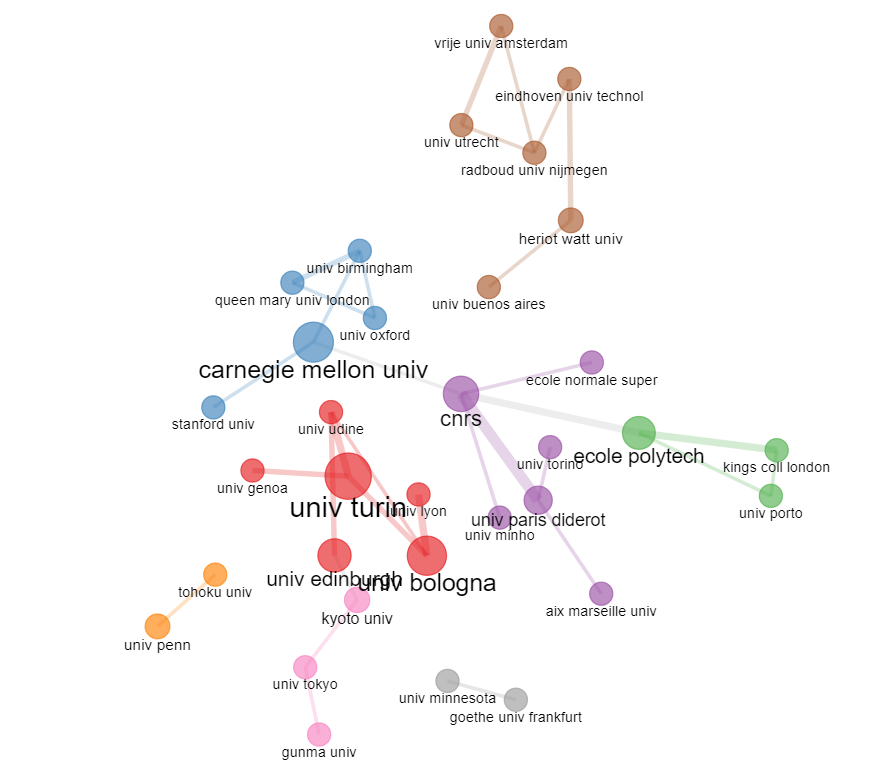
\includegraphics[width=1\textwidth]{experiments/LeoRiether/AnaliseBibliometrica/LambdaCalculus/WoS-20220208/Images/CollaborationNetwork.png}
    \caption{Grafo de colaborações entre instituições no \dataset\  LC@LeoRiether}
    \label{fig:LC@LeoRiether:CollaborationNetwork}
\end{figure}

A figura \ref{fig:LC@LeoRiether:CollaborationNetwork} nos mostra um grafo de colaborações entre instituições no \dataset\  LC@LeoRiether. Nela, vemos universidades como a Carnegie Mellon University, americana; University of Turin, italiana; University of Bologna, também italiana; École Polytechnique, francesa; e CNRS, também francesa. Como esperado, as instituições com mais publicações estão situadas nos países que foram vistos no diagrama de \textit{Sankey}.

Também podemos analisar os graus de cada nó desse grafo (cada colaboração gera uma aresta entre as duas instituições participantes). O gráfico que mostra isso é visto na figura \ref{fig:LC@LeoRiether:CollaborationNetworkDegrees}. Vemos que a distribuição dos graus é exponencial, com poucas instituições com muitas colaborações, e muitas instituições com poucas colaborações.

\begin{figure}
    \centering
    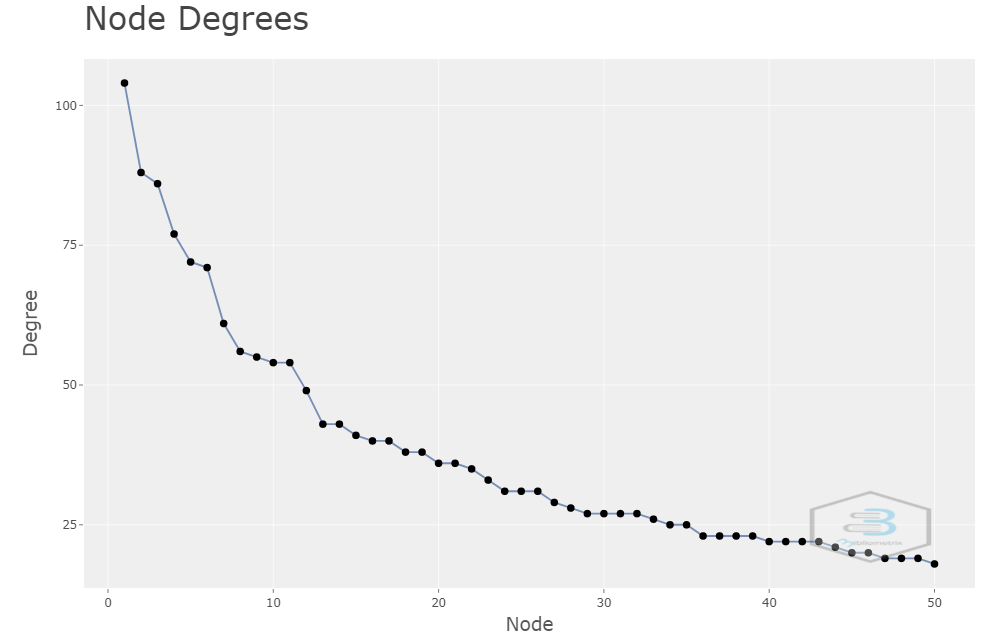
\includegraphics[width=1\textwidth]{experiments/LeoRiether/AnaliseBibliometrica/LambdaCalculus/WoS-20220208/Images/CollaborationNetworkDegrees.png}
    \caption{Quantidade de colaborações de cada nó da rede}
    \label{fig:LC@LeoRiether:CollaborationNetworkDegrees}
\end{figure}

\section{Conclusões}
Foi feita um estudo bibliométrico sobre o estudo científico do cálculo-$\lambda$, utilizando as ferramentas Bibliometrix e Biblioshiny. Com os dados obtidos da Web of Science, foi possível extraír diversas informações sobre essa área da computação.

Nesse estudo, foram analisados vários aspectos dessa área de estudo. Em primeiro lugar, foi analisada a evolução da intensidade de publicações sobre o cálculo-$\lambda$, e foi possível verificar que há um aumento constante nessa intensidade, apesar dela não ser exponencial, como em outras áreas. Além disso, vimos os principais países e instituições que participam do produção científica dessa área, contrastando com quais sub-áreas ou áreas relacionadas elas mencionam em seus artigos. Por último, vimos quais termos e expressões importantes são mencionados em artigos de lambda cálculo, e portanto devem estar relacionados com a área.
